\documentclass[11pt]{amsart}
\usepackage[T1]{fontenc}
\usepackage{lmodern}
\usepackage[margin=1.1in]{geometry}
\usepackage{amsmath,amssymb,mathtools}
\usepackage[expansion=false]{microtype}
\usepackage{enumitem}
\usepackage{booktabs}
\usepackage{tikz}
\usepackage[colorlinks=true,linkcolor=blue,citecolor=blue,urlcolor=blue]{hyperref}
\usepackage[capitalise,noabbrev,nameinlink]{cleveref}
\hypersetup{
  pdftitle={Sharp One-Third Stability of Brenier Maps},
  pdfauthor={OpenAI},
  pdfsubject={Uniform Wasserstein stability for quadratic optimal transport},
  pdfkeywords={optimal transport, Brenier maps, convex potentials, stability}
}
\newcommand{\R}{\mathbb R}
\newcommand{\E}{\mathbb E}
\newcommand{\id}{\mathrm{id}}
\DeclareMathOperator{\Lip}{Lip}
\DeclareMathOperator{\supp}{supp}
\DeclareMathOperator{\Prob}{Prob}
\DeclareMathOperator{\diam}{diam}
\DeclareMathOperator{\Var}{Var}
\newtheorem{theorem}{Theorem}[section]
\newtheorem{lemma}[theorem]{Lemma}
\newtheorem{proposition}[theorem]{Proposition}
\newtheorem{corollary}[theorem]{Corollary}
\theoremstyle{definition}
\newtheorem{definition}[theorem]{Definition}
\theoremstyle{remark}
\newtheorem{remark}[theorem]{Remark}
\numberwithin{equation}{section}
\title[Sharp stability of Brenier maps]{Sharp One-Third Stability of Brenier Maps}
\author{OpenAI}
\date{September 25, 2026}
\begin{document}
\begin{abstract}
For the uniform probability measure \(\rho\) on a compact convex body in
\(\R^d\), \(d\ge2\), quadratic optimal transport maps are one-third
H\"older continuous in \(L^2(\rho)\) with respect to the target's
\(2\)-Wasserstein distance. The constant is uniform over all targets supported in a fixed
compact set, and the exponent is optimal.
A three-atom family on a fixed cube disproves Letrouit's conjectured
uniform square-root estimate.
\end{abstract}
\maketitle
\tableofcontents

\section{Introduction}

Fix an integer \(d\ge2\), a compact convex set \(K\subset\R^d\) with
nonempty interior, and the uniform probability measure
\[
 \rho=\frac{1_K}{|K|}\,dx.
\]
For a nonempty compact set \(Y\subset\R^d\), let \(\Prob(Y)\) denote the
Borel probability measures supported on \(Y\). The quadratic optimal
transport map from \(\rho\) to \(\mu\in\Prob(Y)\) is denoted by \(T_\mu\).
It minimizes
\[
 \int_K |x-T(x)|^2\,d\rho(x)
 \quad\text{subject to }T_\#\rho=\mu
\]
and is unique up to a \(\rho\)-null set. Such maps are gradients of convex
potentials, as in Brenier's theorem \cite{Brenier1991}. We give direct
existence and uniqueness arguments for the maps used here.

For probability measures \(\mu,\nu\) with compact support, write
\[
 W_2(\mu,\nu)
 =\inf_{\pi\in\Pi(\mu,\nu)}
   \left(\int_{\R^d\times\R^d}|y-z|^2\,d\pi(y,z)\right)^{1/2},
\]
where \(\Pi(\mu,\nu)\) is the set of probability couplings. We use
\(W_1(\mu,\nu)=\inf_{\pi\in\Pi(\mu,\nu)}\int|y-z|\,d\pi\)
only when comparing earlier bounds. Our result is the following uniform
estimate.

\begin{theorem}\label{main:stability}
For every \(K,Y\) as above there is a finite constant \(C(K,Y)\) such that
\[
 \|T_\mu-T_\nu\|_{L^2(\rho)}
 \le C(K,Y)\,W_2(\mu,\nu)^{1/3}
 \qquad\bigl(\mu,\nu\in\Prob(Y)\bigr).
\]
The targets may be atomic, singular, or absolutely continuous. The
exponent \(1/3\) cannot be replaced by any larger exponent in general,
even for \(K=Y=[-1,1]^d\) and targets with exactly three atoms.
\end{theorem}

The constant is independent of atom count, positive atom masses, site
separation, and density bounds. Neither smoothness nor strict convexity
of \(K\) is required, and \(Y\) need not be convex. An explicit admissible
constant is obtained in \Cref{gradient:finite}.

\subsection{History and significance}

Quantitative stability asks how strongly the representation of a target
measure by its optimal map depends on the target. Earlier contributions
include Ambrosio's local one-half H\"older estimate along target curves
near regular data, reported by Gigli
\cite[Corollary~3.4]{Gigli2011}, and Berman's estimates for varying
sources against a fixed target whose density is bounded below on a
convex domain \cite{Berman2021}. M\'erigot, Delalande, and Chazal
used dualization to obtain target-uniform bounds from Berman's work,
with dimension-dependent exponents, and then proved a
dimension-independent \(W_1^{2/15}\) bound for a uniform convex source
\cite[Corollary~2.4 and Theorem~3.1]{MerigotDelalandeChazal2020}.

Potential estimates followed by convex-gradient interpolation became
central to the target-uniform problem. Delalande and M\'erigot proved
an \(L^2\)-map bound of order \(W_1^{1/6}\) for source densities bounded
above and below on a convex domain and targets in a fixed compact set
\cite[Theorem~4.2]{DelalandeMerigot2023}. Their interpolation inequality
\cite[Proposition~4.1]{DelalandeMerigot2023} is the antecedent of our
last step; the improvement here is the linear \(W_2\) estimate for
potential differences. Letrouit and M\'erigot extended potential
stability to John domains by local-to-global variance arguments, and
obtained the corresponding map estimate when the boundary is
rectifiable with finite \((d-1)\)-dimensional measure
\cite[Theorem~1.7]{LetrouitMerigot2024}.

Divol, Niles-Weed, and Pooladian obtained a
\(W_2^{1/3}\)-map estimate for regular source densities and
nondegenerate finite targets
\cite[Theorem~4.3]{DivolNilesWeedPooladian2025}. Its constant depends on
the number of atoms, a positive lower bound for their masses, and
separation and angular geometry, whereas \Cref{main:stability} has one
constant for all Borel targets, including degenerating atomic measures.
At the other end of the regularity scale, Lipschitz \(L^2\) stability
in \(W_2\) holds for uniformly positive H\"older-continuous densities
on suitably regular uniformly convex domains
\cite[Theorem~1.1]{CajaLopezDelgadinoKitagawa2026}. Its constants depend
on nondegeneracy and regularity conditions that exclude our atomic
targets.

Cazelles, Pauwels, and Portales obtained a \(W_1^{1/5}\) map bound for
bounded source densities and compactly supported marginals in their
analysis of Monge-map estimation
\cite[Corollary~4.9]{CazellesPauwelsPortales2026}.
Han and Zhu \cite[Proposition~2.7]{HanZhu2026} report a sharp
\(W_1^{1/4}\) estimate of M\'erigot \cite{Merigot2026}; see also
\cite[Section~2.3]{ChewiEichingerPooladian2026}. Since \(W_1\le W_2\),
a quarter-power estimate in \(W_1\) gives at most a quarter-power
estimate in \(W_2\) by that comparison alone. In the fixed-cube family
of \Cref{sharpness:exponent}, \(W_1\) and \(W_2\) have different scaling,
so its \(W_2^{1/3}\) obstruction is compatible with a sharp
\(W_1^{1/4}\) estimate.

Letrouit proved an obstruction to exponents above \(1/3\) for a
nonconvex source and formulated uniform square-root stability in \(W_2\)
for a uniform convex source as a conjecture
\cite[Theorem~2 and Conjecture~3]{Letrouit2026}. The fixed-cube
three-plane construction proved in \Cref{sharpness:exponent} disproves
that conjectured exponent and every other exponent above \(1/3\), even
with only three target atoms. The positive bound in \Cref{main:stability}
identifies the matching uniform endpoint. Together, the two parts
determine the sharp exponent within the stated uniform-source class.

\subsection{Sharpness and the finite-cell argument}

We begin in \Cref{sec:sharpness} with the obstruction. A maximum of
three affine functions has a thin central cell between two outer cells.
Tilting the middle affine function preserves its cell mass but switches
source points between slopes at order-one separation. The resulting
three-atom targets give the sharpness assertion. The remaining sections
prove the matching upper bound.

For distinct sites \(y_1,\ldots,y_N\) and intercepts
\(c=(c_1,\ldots,c_N)\), set
\[
 u_c(x)=\max_i\{x\cdot y_i+c_i\},\qquad
 P_i(c)=\{x\in K:u_c(x)=x\cdot y_i+c_i\}.
\]
The cells partition \(K\) up to null sets, and \(\nabla u_c=y_i\)
almost everywhere on cell \(i\). Write
\(M_i(c)=\rho(P_i(c))\) and
\(B_i(c)=\int_{P_i(c)}x\,d\rho(x)\) for its mass and first moment.
\Cref{sec:cells} establishes the cell calculus and shows that the
intercepts realizing prescribed positive masses depend differentiably
on the sites. At a configuration with all \(M_i>0\), fix
\(q\in\R^N\) and let dots denote derivatives along \(c+s q\) at
\(s=0\), with the sites fixed.
The central estimate, proved in \Cref{sec:moments}, is
\[
 \sum_i\frac{|\dot B_i|^2}{M_i}
 \le C_0R^2\sum_i\frac{|\dot M_i|^2}{M_i},
 \qquad K\subset B(0,R),
\]
with an absolute constant \(C_0\). Couple the uniform laws on the cells
at \(c-s q\) and \(c+s q\). Their midpoint law, multiplied by the
geometric mean of their masses, can be dominated by the source measure
on the cell at \(c\). We prove this density bound by Knothe's triangular
rearrangement \cite{Knothe1957}; it is also a consequence of displacement
concavity \cite[Theorem~2.3]{McCann1997}. Testing with
\(R^2-|x|^2\) and summing over the partitions controls displacement by
mass changes. This produces the moment estimate with a constant that
remains uniform as masses or faces become small.

In \Cref{sec:finite-stability}, we move the sites of two finite targets
along an optimal target coupling while keeping the coupling masses
fixed. The derivative of the cell-mass constraint is a graph-Laplacian
equation, familiar from semi-discrete transport
\cite{KitagawaMerigotThibert2019}. We test it against an intercept
direction whose mass derivative is the weighted intercept velocity.
The moment inequality then bounds that velocity directly in its
weighted \(L^2\) norm. This avoids any quantitative bound on the inverse
Laplacian and yields an \(L^2(\rho)\) potential difference of order
\(W_2(\mu,\nu)\).

Finally, \Cref{sec:gradient} uses coordinate slices to bound the squared
gradient difference by a constant times
\[
 h^{-2}\|u_0-u_1\|_{L^2(\rho)}^2+h.
\]
The potential estimate and the choice \(h=W_2(\mu,\nu)^{2/3}\) give
the one-third exponent. Finite approximation and supporting inequalities
then extend the estimate to all Borel targets. The source's convexity
enters through its convex cells and interval slices; no smoothness of
its boundary is used.

\subsection{Conventions}

Lebesgue volume is denoted by \(|\cdot|\), and surface measure on an affine
hyperplane by \(dS\). All source masses and moments are normalized by
\(|K|\). We choose fixed \(R,L\ge1\) such that
\(K\subset B(0,R)\) and \(Y\subset B(0,L)\). A finite maximum of affine
functions with slopes in \(B(0,L)\) is convex and \(L\)-Lipschitz.
Ties between distinct slopes occur on a finite union of hyperplanes and
therefore have zero source measure.

\section{Sharpness on a fixed cube}
\label{sec:sharpness}

We first prove that the exponent in \Cref{main:stability} cannot be
improved. The example uses three affine functions, with a small change
in one slope reassigning source points between the central and outer
cells. The following observation identifies the resulting gradients as
optimal maps. It applies to the general source body $K$ of the introduction.

\begin{lemma}[Optimality of a finite affine maximum]
\label{cells:optimality}
Let
\[
 u(x)=\max_{1\le i\le N}\bigl(x\cdot y_i+c_i\bigr).
\]
For $\rho$-almost every $x$, all maximizing indices have the same slope.
Define $T(x)=y_i$ for the smallest maximizing index $i$, and put
$\lambda=T_\#\rho$. Then $T$ is Borel, $T=\nabla u$ almost everywhere, and
the transport plan $(\id,T)_\#\rho$ is the unique quadratic-cost optimal
plan from $\rho$ to $\lambda$.
\end{lemma}

\begin{proof}
The first-index choice is Borel because its level sets are given by
finitely many strict and non-strict affine inequalities.
Merge repeated slopes, retaining the largest intercept for each slope, and
write the resulting intercept as $c(y)$. Ties between distinct slopes lie
in a finite union of hyperplanes. Outside this null set, the maximizing
affine function remains strictly maximal in a neighborhood, so its slope
is the gradient of $u$.

For every transport plan $\pi$ from $\rho$ to $\lambda$, the inequality
$x\cdot y+c(y)\le u(x)$ gives
\[
 \int x\cdot y\,d\pi(x,y)
 \le \int_K u\,d\rho-\int c(y)\,d\lambda(y).
\]
The graph plan of $T$ attains equality. Since the two marginals fix the
integrals of $|x|^2$ and $|y|^2$, maximizing the displayed scalar product is
equivalent to minimizing quadratic cost. Equality for any optimal plan
requires it to be concentrated on pairs $(x,y)$ with
$x\cdot y+c(y)=u(x)$. The maximizing slope is unique for $\rho$-almost every
$x$, so the plan is concentrated on the graph of $T$. This proves
uniqueness of the plan.
\end{proof}

We now specialize to the cube. The two targets below have the same atom
masses, but their optimal maps differ on a much larger part of the source
than their target displacement alone might suggest.

\begin{proposition}[Optimality of the exponent]\label{sharpness:exponent}
For every fixed $d\ge2$, let $K=Y=[-1,1]^d$ and
$\rho=2^{-d}1_K\,dx$.  For every $\alpha>1/3$,
\[
 \sup_{\substack{\mu,\nu\in\Prob(Y)\\ \mu\ne\nu}}
 \frac{\|T_\mu-T_\nu\|_{L^2(\rho)}}{W_2(\mu,\nu)^\alpha}
 =+\infty.
\]
The supremum remains infinite when both targets are required to have
exactly three atoms.
\end{proposition}

\begin{proof}
For $0<a<1/2$, put $b=a/2$ and define
\begin{equation}\label{sharpness:potentials}
 u_a(x)=\max\{-x_1,x_1,a\},\qquad
 \widetilde u_a(x)=\max\{-x_1,x_1,a+bx_2\}.
\end{equation}
Let $\mu_a=(\nabla u_a)_\#\rho$ and
$\nu_a=(\nabla\widetilde u_a)_\#\rho$, with any fixed first-index
selection on the null tie sets.  Their slopes are, respectively,
$-e_1,e_1,0$ and $-e_1,e_1,be_2$, all in the fixed set $Y$.
By \Cref{cells:optimality}, these gradients are the unique optimal
maps to their laws.

Since $a/2\le a+bx_2\le3a/2<1$, the central cells are, up to null
boundaries,
\[
 A_a=\{x\in K:|x_1|<a\},\qquad
 B_a=\{x\in K:|x_1|<a+bx_2\}.
\]
Tilting the central strip preserves its mass but changes which points
receive a central or an outer slope. \Cref{fig:sharpness-cells} shows
the symmetric difference where this reassignment occurs.

\begin{figure}[tbp]
\centering
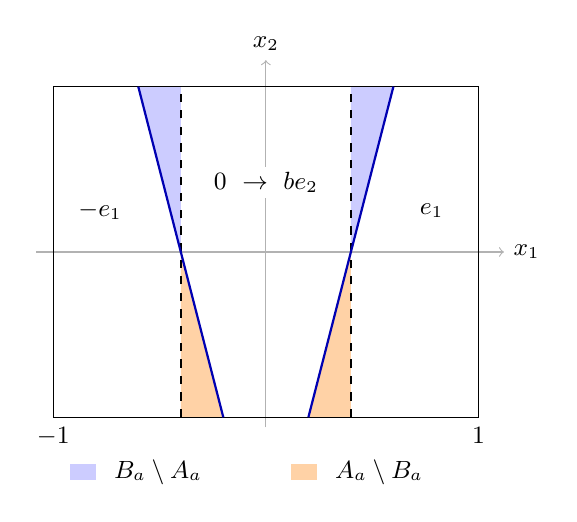
\begin{tikzpicture}[x=2.7cm,y=2.1cm,font=\small]
 \fill[blue!20] (-0.4,0)--(-0.6,1)--(-0.4,1)--cycle;
 \fill[blue!20] (0.4,0)--(0.6,1)--(0.4,1)--cycle;
 \fill[orange!35] (-0.4,0)--(-0.4,-1)--(-0.2,-1)--cycle;
 \fill[orange!35] (0.4,0)--(0.4,-1)--(0.2,-1)--cycle;
 \draw[gray!60,->] (-1.08,0)--(1.12,0) node[right,text=black] {$x_1$};
 \draw[gray!60,->] (0,-1.06)--(0,1.16) node[above,text=black] {$x_2$};
 \draw (-1,-1) rectangle (1,1);
 \draw[dashed,thick] (-0.4,-1)--(-0.4,1);
 \draw[dashed,thick] (0.4,-1)--(0.4,1);
 \draw[blue!70!black,thick] (-0.2,-1)--(-0.6,1);
 \draw[blue!70!black,thick] (0.2,-1)--(0.6,1);
 \node[fill=white,inner sep=2pt] at (-0.78,0.25) {$-e_1$};
 \node[fill=white,inner sep=2pt] at (0.78,0.25) {$e_1$};
 \node[fill=white,inner sep=2pt] at (0,0.42) {$0\ \to\ be_2$};
 \node[below] at (-1,-1) {$-1$};
 \node[below] at (1,-1) {$1$};
 \fill[blue!20] (-0.92,-1.38) rectangle (-0.8,-1.28);
 \node[right] at (-0.76,-1.33) {$B_a\setminus A_a$};
 \fill[orange!35] (0.12,-1.38) rectangle (0.24,-1.28);
 \node[right] at (0.28,-1.33) {$A_a\setminus B_a$};
\end{tikzpicture}
\caption{A source-coordinate section of the cube example, drawn with
$a=2/5$ and $b=a/2$. Dashed lines bound $A_a$; solid blue lines bound
$B_a$. The two shaded sets have equal area, so the central mass stays
fixed. On their union, source points switch between central and outer
slopes. The labels show map values on the unchanged outer regions and
the common central region; they are not target points plotted in the
source plane. The remaining coordinates integrate out.}
\label{fig:sharpness-cells}
\end{figure}

On $A_a$, the first map is zero; on its complement it is
$\operatorname{sign}(x_1)e_1$.  The second map equals $be_2$ on
$B_a$ and $\operatorname{sign}(x_1)e_1$ on its complement.
Under $\rho$, the coordinates are independent and uniform on
$[-1,1]$.  On the slice $x_2=t$, the second central interval has
probability $a+bt$, and each outer interval has probability
$(1-a-bt)/2$.  Averaging over $t$ gives
\begin{equation}\label{sharpness:targets}
 \mu_a=\frac{1-a}{2}(\delta_{-e_1}+\delta_{e_1})+a\delta_0,
 \qquad
 \nu_a=\frac{1-a}{2}(\delta_{-e_1}+\delta_{e_1})+a\delta_{be_2}.
\end{equation}
Both targets have three distinct atoms of positive mass.

The coupling that fixes the outer atoms and moves the central atom
from $0$ to $be_2$ has squared cost $ab^2$.  Conversely, every point
in the support of $\mu_a$ has second coordinate zero.  Every coupling
$\pi$ of the two targets therefore satisfies
\[
 \int|y-z|^2\,d\pi(y,z)
 \ge\int|y_2-z_2|^2\,d\pi(y,z)=ab^2.
\]
Consequently,
\begin{equation}\label{sharpness:target-distance}
 W_2(\mu_a,\nu_a)^2=ab^2.
\end{equation}
The same matching coupling costs $ab$ for $W_1$, while every coupling
has cost at least
$\int|y_2-z_2|\,d\pi=ab$. Thus
\begin{equation}\label{sharpness:w1-distance}
 W_1(\mu_a,\nu_a)=ab=\frac{a^2}{2}.
\end{equation}

The two central intervals on the slice $x_2=t$ are nested, and their
symmetric difference has conditional probability $b|t|$.  Thus
\[
 \rho(A_a\mathbin{\triangle}B_a)
 =\frac12\int_{-1}^1b|t|\,dt=\frac b2.
\]
The first coordinate of the map difference contributes the indicator
of that symmetric difference, and its second coordinate contributes
$b^2$ on $B_a$.  Orthogonality gives the pointwise identity
\[
 |T_{\mu_a}-T_{\nu_a}|^2
 =1_{A_a\mathbin{\triangle}B_a}+b^2 1_{B_a}
 \quad\rho\hbox{-almost everywhere}.
\]
Since $\rho(B_a)=a$, this proves
\begin{equation}\label{sharpness:map-distance}
 \|T_{\mu_a}-T_{\nu_a}\|_{L^2(\rho)}^2=\frac b2+ab^2.
\end{equation}
The remaining $d-2$ coordinates integrate out, so all computations
hold in every fixed dimension $d\ge2$.

Substituting $b=a/2$ into \eqref{sharpness:target-distance} and
\eqref{sharpness:map-distance} gives
\[
 W_2(\mu_a,\nu_a)=\frac{a^{3/2}}2,
 \qquad
 \|T_{\mu_a}-T_{\nu_a}\|_{L^2(\rho)}
 =\frac{\sqrt a}{2}\sqrt{1+a^2}.
\]
For every $\alpha>1/3$, their ratio is
\[
 \frac{\|T_{\mu_a}-T_{\nu_a}\|_{L^2(\rho)}}
      {W_2(\mu_a,\nu_a)^\alpha}
 =2^{\alpha-1}\sqrt{1+a^2}\,a^{(1-3\alpha)/2}
 \longrightarrow+\infty\qquad(a\downarrow0).
\]
The source, target container, and number of atoms stay fixed,
proving the proposition.
\end{proof}

\section{Finite affine potentials and prescribed cell masses}
\label{sec:cells}

We return to an arbitrary compact convex body $K\subset\R^d$ and its
uniform probability measure $\rho=\mathbf 1_K\,dx/|K|$. To compare targets
by moving their sites, we need intercepts that keep prescribed cell masses
fixed and depend differentiably on the sites. We first compute the derivatives
of cell masses and moments, then use them to construct these intercepts.

Assume that the sites $y_1,\ldots,y_N$ are distinct. For intercepts
$c=(c_1,\ldots,c_N)$, set
\begin{align*}
 P_i&=K\cap\bigcap_{j\ne i}
 \{x:x\cdot(y_i-y_j)+c_i-c_j\ge0\},\\
 M_i&=\rho(P_i),
 &B_i&=\int_{P_i}x\,d\rho(x).
\end{align*}
These closed convex cells partition $K$ up to the null tie set. Denote the
equality plane and the common face by
\[
 H_{ij}=\{x:x\cdot(y_i-y_j)+c_i-c_j=0\},
 \qquad F_{ij}=P_i\cap P_j.
\]
All integrals over $F_{ij}$ use the $(d-1)$-dimensional measure $dS$ of
$H_{ij}$, so an empty or lower-dimensional face contributes zero. Define
the symmetric coefficients
\begin{equation}
\label{cells:face-coefficients}
 g_{ij}=\frac{1}{|K|\,|y_i-y_j|}\int_{F_{ij}}1\,dS,
 \qquad
 b_{ij}=\frac{1}{|K|\,|y_i-y_j|}\int_{F_{ij}}x\,dS.
\end{equation}

These cells are often called Laguerre cells. Their fixed-site mass
derivative has the standard face-integral and weighted graph-Laplacian
form \cite[Theorem~1.3 and Section~5.3]{KitagawaMerigotThibert2019}.
We include the calculation for the joint site and moment variations
needed here.

\begin{proposition}[Cell differentials and connectivity]
\label{cells:calculus}
On the open set of configurations with distinct sites and $M_i>0$ for
every $i$, the maps $M_i$ and $B_i$ are jointly $C^1$ in the intercepts and
sites. For an intercept direction $r=(r_i)$ and a site direction
$v=(v_i)$,
\begin{align}
 D M_i[r,v]
 &=\sum_{j\ne i}\bigl[g_{ij}(r_i-r_j)
          +b_{ij}\cdot(v_i-v_j)\bigr],
 \label{cells:mass-differential}\\
 D B_i[r,v]
 &=\sum_{j\ne i}b_{ij}(r_i-r_j)
   +\frac1{|K|}\sum_{j\ne i}\frac1{|y_i-y_j|}
        \int_{F_{ij}}x\bigl(x\cdot(v_i-v_j)\bigr)\,dS(x).
 \label{cells:moment-differential}
\end{align}
The graph on $\{1,\ldots,N\}$ with edges $g_{ij}>0$ is connected.
Consequently, the symmetric operator
\begin{equation}
\label{cells:laplacian}
 (Gq)_i=D M_i[q,0]=\sum_{j\ne i}g_{ij}(q_i-q_j)
\end{equation}
has kernel consisting of the constant vectors and range
$\{z\in\R^N:\sum_i z_i=0\}$.
\end{proposition}

\begin{proof}
We first record the geometric facts that permit differentiation for an
arbitrary convex body. The boundary of a full-dimensional compact convex
set has zero volume: contractions toward an interior point lie in the
interior and their volumes tend to the full volume. The same argument
applies within an affine subspace. Moreover, if a hyperplane $H$ meets
$\operatorname{int}K$, then
\[
 \operatorname{relint}(K\cap H)=\operatorname{int}K\cap H.
\]
Indeed, choose $p\in\operatorname{int}K\cap H$. A relative interior point
$z\ne p$ of the section lies strictly between $p$ and a point of the
section beyond $z$. A strict convex combination with the ambient interior
point $p$ lies in $\operatorname{int}K$. The reverse inclusion is immediate.
It follows that $\partial K\cap H$ has zero $(d-1)$-dimensional measure.

Since $M_i>0$, cell $i$ contains an interior point of $K$ at which its
affine function is strictly maximal: remove the boundary of $K$ and the
finite union of tie planes from the positive-volume cell. Strictly active
points for $i$ and $j$ give opposite signs of their affine difference, so
$H_{ij}$ meets $\operatorname{int}K$. Also, $H_{ij}$ and $H_{ik}$ cannot
coincide for three distinct indices. Coincidence would make their affine
differences proportional. The three affine functions would then lie on
one affine line, with one a strict convex combination of the other two;
that function could never be strictly maximal. Hence the intersections
$H_{ij}\cap H_{ik}$ are empty or have dimension at most $d-2$.

We next prove the differential formulas. For a continuous function
$f:\R^d\to\R$, write
\[
 I_i^f=\frac1{|K|}\int_K f(x)
        \prod_{j\ne i}\mathbf1_{\{\ell_{ij}(x)\ge0\}}\,dx,
 \qquad
 \ell_{ij}(x)=x\cdot(y_i-y_j)+c_i-c_j.
\]
Only $f=1$ and $f(x)=x_k$ will be needed. Perturb $(c,y)$ by $h(r,v)$,
with $h\downarrow0$, and telescope the difference of the products of
indicators one factor at a time. On bounded $K$, the term in which the
$j$-th factor changes is supported in
$|\ell_{ij}(x)|\le Ch$, with $C$ fixed for the configuration and direction.
Put $n_{ij}=(y_i-y_j)/|y_i-y_j|$ and use coordinates
\[
 x=z+htn_{ij},\qquad z\in H_{ij}.
\]
Both $z$ and $t$ can be restricted to fixed bounded sets. The factor $h$
in the volume element cancels the difference quotient. Outside
\[
 (\partial K\cap H_{ij})
 \ \cup\!\bigcup_{k\ne i,j}(H_{ik}\cap H_{ij}),
\]
a surface-null set by the preceding geometric observations, all remaining
indicators converge to their values at $z$. The changed factor converges
for almost every $(z,t)$ to
\[
 \mathbf1_{\{|y_i-y_j|t+r_i-r_j+z\cdot(v_i-v_j)\ge0\}}
       -\mathbf1_{\{t\ge0\}}.
\]
Its integral in $t$ is
$(r_i-r_j+z\cdot(v_i-v_j))/|y_i-y_j|$. Dominated convergence therefore gives
\begin{equation}
\label{cells:general-differential}
 D I_i^f[r,v]
 =\frac1{|K|}\sum_{j\ne i}\frac1{|y_i-y_j|}
    \int_{F_{ij}} f(z)
       \bigl(r_i-r_j+z\cdot(v_i-v_j)\bigr)\,dS(z).
\end{equation}
Applying the same argument in the opposite direction supplies the
two-sided derivative. Taking $f=1,x_1,\ldots,x_d$ gives
\eqref{cells:mass-differential} and \eqref{cells:moment-differential}.

For completeness, these derivatives are continuous under joint changes
of sites and intercepts. Identify a nearby equality plane with the fixed
$H_{ij}$ as an affine graph in the normal direction $n_{ij}$. The graph
maps and their surface Jacobians converge uniformly on a common bounded
integration region. The face-defining indicators converge outside the
same surface-null sets used above. The remaining integrands and the
positive denominators $|y_i-y_j|$ converge as well. Dominated convergence
proves continuity of each coefficient of the differential, including
those containing $z_kz_l$. Thus all coordinate partial derivatives exist
and are continuous, which yields joint $C^1$ regularity. The admissible
parameter set is open: the masses themselves are continuous by dominated
convergence away from the original tie hyperplanes.

To prove connectivity, fix strictly active interior points in any two
cells. They may be chosen so that the first point $p$ avoids all equality
planes and the second point $q$ avoids all equality planes and the affine
spans of $p$ with every triple equality set. These are finitely many
proper affine subsets, so they cannot cover a strictly active open
region. The segment $[p,q]$ lies in $\operatorname{int}K$ and meets no
triple equality set. At any change of active index along it, precisely
two affine functions are maximal. The other inequalities are strict,
so a small relatively open disk in their equality plane belongs to the
common face. That face has positive area and gives an edge of the graph.
The successive active indices therefore give a graph path between the
chosen cells.

Finally, symmetry of the face coefficients gives
\[
 q\cdot Gq=\sum_{i<j}g_{ij}(q_i-q_j)^2.
\]
Connectivity identifies the kernel as the constant vectors. Symmetry
then identifies the range as their orthogonal complement, as claimed.
\end{proof}

\begin{proposition}[Prescribed cell masses]
\label{cells:weights}
Fix positive weights $m_1,\ldots,m_N$ with $\sum_i m_i=1$. For every
configuration of distinct sites, there is a unique vector of intercepts
$c$ satisfying
\begin{equation}
\label{cells:prescribed-masses}
 M_i=m_i\quad(1\le i\le N),\qquad \sum_i m_i c_i=0.
\end{equation}
With the weights fixed, this normalized vector is a $C^1$ function of
the sites on the open set of distinct-site configurations.
\end{proposition}

\begin{proof}
The case $N=1$ has $c_1=0$, so assume $N\ge2$. On the normalization space
$H_m=\{c\in\R^N:\sum_i m_i c_i=0\}$, minimize the convex function
\[
 \mathcal F_y(c)=\int_K\max_i(x\cdot y_i+c_i)\,d\rho(x)
                  -\sum_i m_i c_i.
\]
Choose $R$ with $|x|\le R$ on $K$, and set $S=\max_i|y_i|$. On $H_m$,
\[
 \mathcal F_y(c)\ge\max_i c_i-RS.
\]
Positivity of all the weights implies that $\max_i c_i$ tends to infinity
as $|c|\to\infty$ within $H_m$: an upper bound on all coordinates and the
weighted mean-zero identity also bound every coordinate below. Hence
$\mathcal F_y$ is coercive on $H_m$ and attains its minimum.

Distinct sites give an almost-everywhere unique maximizing index for
every $c$. Differentiation of the maximum under the integral, justified
by bounded difference quotients, shows
\[
 \nabla_c\mathcal F_y=(M_i-m_i)_{i=1}^N.
\]
At a minimum on $H_m$, this gradient lies in $\operatorname{span}\{m\}$.
Its coordinate sum is zero because the masses and weights each sum to
one. Since $\sum_i m_i=1$, the gradient must vanish. Thus a normalized
solution of \eqref{cells:prescribed-masses} exists. Conversely, every such
solution is a minimizer by convexity.

At any solution all cells have positive mass, so \Cref{cells:calculus}
applies. The intercept derivative of the mass residual is the restriction
\[
 G:H_m\longrightarrow H_0,
 \qquad H_0=\{z\in\R^N:\textstyle\sum_i z_i=0\}.
\]
It is an isomorphism: both spaces have dimension $N-1$, and the only
constant vector in $H_m$ is zero. The finite-dimensional implicit
function theorem therefore gives a locally unique $C^1$ solution as the
sites vary. In particular, each solution is locally isolated for its
fixed sites. If two normalized solutions existed, their segment would
consist of minimizers of the convex objective, contradicting this local
isolation. Global uniqueness follows, and the local $C^1$ solution
branches agree wherever they overlap. This proves the claimed $C^1$
dependence on the sites. Only the invertibility of the restricted
Laplacian is used here; no quantitative bound on its inverse is needed.
\end{proof}

\section{A uniform estimate for cell moments}
\label{sec:moments}

We compare changes in the first moments and masses of cells when their
intercepts vary and their sites remain fixed. The estimate is uniform
over all configurations with positive cell masses.

\begin{lemma}[Stationary-site moment estimate]\label{moments:derivative}
Fix distinct sites $y_1,\ldots,y_N$ and intercepts $c_1,\ldots,c_N$
whose cells have positive masses $M_i$. If $K\subset\{x:|x|\le R\}$,
then every intercept direction $q\in\R^N$ satisfies
\[
  \sum_{i=1}^N\frac{|D B_i[q,0]|^2}{M_i}
  \le C_0R^2\sum_{i=1}^N\frac{|D M_i[q,0]|^2}{M_i},
  \qquad C_0=162.
\]
\end{lemma}

The proof couples uniform laws on two opposite perturbations of each
cell. Their midpoint lies in the original cell; the following lemma
controls its density.

\begin{lemma}[Midpoint coupling]\label{moments:midpoint}
Let $U,V\subset\R^d$ be compact convex sets of positive volume. There is a
coupling $(X,Z)$ of the uniform probability measures on $U$ and $V$ such that
\[
  \operatorname{Law}\!\left(\frac{X+Z}{2}\right)
  \le \frac{dx}{\sqrt{|U||V|}}.
\]
The inequality is an inequality of measures on $\R^d$.
\end{lemma}

This density bound also follows from McCann's displacement-concavity
inequality \cite[Theorem~2.3]{McCann1997}. We give a direct proof by the
conditional-quantile construction underlying Knothe's triangular
rearrangement \cite{Knothe1957,CarlierGalichonSantambrogio2010}.
The subsequent application to cell moments is developed here.

\begin{proof}
We parameterize the two uniform laws by successive one-dimensional
quantiles on the same cube. Their diagonal derivatives have constant
products. Averaging the two maps and substituting coordinates successively
will give the density bound.

We need the boundary observation from the proof of \Cref{cells:calculus}
for arbitrary positive-dimensional affine slices, not only hyperplanes.
The same segment-extension argument shows that a relative interior point
of a slice of $U$ meeting $\operatorname{int}U$ is an ambient interior
point: unless it equals a chosen ambient interior point in the slice,
it lies strictly between that point and a farther point of the section.
The contraction argument for convex
boundaries, applied within the slice, then shows that its intersection
with $\partial U$ has zero slice volume.

For $0\le k<d$, let
\[
  p_k(\xi)=\int_{\R^{d-k}}
       1_{\operatorname{int}U}(\xi,\eta)\,d\eta,
  \qquad
  p_d=1_{\operatorname{int}U}.
\]
Thus $p_0=|U|$. Write $D_k$ for the projection of
$\operatorname{int}U$ onto its first $k$ coordinates. Each $p_k$ is
positive and continuous on $D_k$. For $k<d$, continuity follows by
dominated convergence: at a prefix in $D_k$, the preceding boundary
property makes the indicators of the fibers converge almost everywhere
as the prefix varies, and boundedness of $U$ provides a common integrable
bound. For $k=d$ the assertion is immediate. The fiber integrals are
Borel functions on their full domains.

Given $s=(s_1,\ldots,s_d)\in(0,1)^d$, construct $X(s)$ recursively.
For a previously constructed prefix
$\xi=(X_1,\ldots,X_{k-1})\in D_{k-1}$, let $X_k$ be the quantile
at level $s_k$ of the density
\[
  t\longmapsto \frac{p_k(\xi,t)}{p_{k-1}(\xi)}.
\]
Fubini's theorem shows that this density integrates to one. It is
positive and continuous on the bounded open interval
$\{t:(\xi,t)\in D_k\}$, and vanishes outside that interval.
Its cumulative distribution function is therefore strictly increasing
from zero to one there. This defines the quantile uniquely, keeps the
new prefix in $D_k$, and gives
\[
  \partial_{s_k}X_k
   =\frac{p_{k-1}(X_1,\ldots,X_{k-1})}
          {p_k(X_1,\ldots,X_k)}>0.
\]
For each fixed earlier parameter prefix, $X_k$ is $C^1$ in $s_k$.
The conditional cumulative distribution functions are Borel in their
arguments, so comparison at rational points shows that their quantiles
are Borel. Thus the whole construction is measurable. With $s$ uniform
on the cube, successive conditioning gives the uniform law on $U$.
The diagonal derivatives telescope to
\[
  \prod_{k=1}^d\partial_{s_k}X_k=|U|.
\]
Construct $Z(s)$ in the same way for $V$, using the same parameters.
For $H=(X+Z)/2$, the arithmetic--geometric mean inequality yields
\[
  \prod_{k=1}^d\partial_{s_k}H_k
  \ge
  \sqrt{\left(\prod_{k=1}^d\partial_{s_k}X_k\right)
              \left(\prod_{k=1}^d\partial_{s_k}Z_k\right)}
  =\sqrt{|U||V|}.
\]

We justify substitution using only the stated regularity in each
coordinate. For a nonnegative Borel function $g$ on $\R^d$, fix
$a=(s_1,\ldots,s_{d-1})$. One-dimensional substitution in the strictly
increasing $C^1$ function $s_d\mapsto H_d(a,s_d)$, followed by enlargement
of its image interval to $\R$, gives
\[
  \int_0^1 g\bigl(H_1(a),\ldots,H_{d-1}(a),H_d(a,t)\bigr)
                 \partial_{s_d}H_d(a,t)\,dt
  \le \int_{\R}g\bigl(H_1(a),\ldots,H_{d-1}(a),z\bigr)\,dz.
\]
Here each $H_k(a)$ uses only the first $k$ entries of $a$.
The integral of $g$ in its last variable is again a nonnegative Borel
function. The earlier derivative factors depend only on earlier
parameters. Tonelli's theorem therefore permits multiplication by their
product and integration in $a$. Repeating this argument backwards gives
\[
  \int_{(0,1)^d}g(H(s))
       \prod_{k=1}^d\partial_{s_k}H_k(s)\,ds
  \le \int_{\R^d}g(x)\,dx.
\]
All derivative factors are Borel, as also follows from their explicit
formulas above. No differentiability in earlier parameters or boundedness
of the derivatives near the boundary of the cube is required.
Combining the last two inequalities proves
\[
  \E g\!\left(\frac{X+Z}{2}\right)
  \le \frac{1}{\sqrt{|U||V|}}\int_{\R^d}g(x)\,dx,
\]
which is the asserted measure domination.
\end{proof}

\begin{proof}[Proof of \Cref{moments:derivative}]
Fix the intercept direction $q$ and hold the sites fixed.
For sufficiently small $s>0$, let $P_i^-$ and
$P_i^+$ be the cells at $c-sq$ and $c+sq$, respectively, and write
\[
  \alpha_i=\rho(P_i^-),\qquad
  \beta_i=\rho(P_i^+),\qquad
  \gamma_i=\sqrt{\alpha_i\beta_i}.
\]
These masses are positive by continuity from \Cref{cells:calculus}.
The perturbed cells are compact convex sets of positive volume.
Couple their uniform probability measures by \Cref{moments:midpoint},
writing $X_i\in P_i^-$, $Z_i\in P_i^+$, and
$D_i=\E|X_i-Z_i|^2$. For each competing index $j$, the defining
inequalities give
\begin{align*}
  X_i\cdot(y_i-y_j)+c_i-c_j-s(q_i-q_j)&\ge0,\\
  Z_i\cdot(y_i-y_j)+c_i-c_j+s(q_i-q_j)&\ge0.
\end{align*}
Averaging shows that $(X_i+Z_i)/2$ satisfies the $i$-cell inequalities
at $c$; convexity also places it in $K$. Its law is supported on $P_i$.
Since $|P_i^-|=|K|\alpha_i$ and $|P_i^+|=|K|\beta_i$, the midpoint
bound has exactly the normalization
\[
  \gamma_i\operatorname{Law}\!\left(\frac{X_i+Z_i}{2}\right)
  \le \frac{1_{P_i}\,dx}{|K|}=\rho|_{P_i}.
\]

Use the nonnegative function $\Phi(x)=R^2-|x|^2$ on $K$, and set
$A_i^-=\E\Phi(X_i)$ and $A_i^+=\E\Phi(Z_i)$. The identity
\[
  \Phi\!\left(\frac{X_i+Z_i}{2}\right)
  =\frac{\Phi(X_i)+\Phi(Z_i)}2+\frac{|X_i-Z_i|^2}{4}
\]
and the cellwise measure domination imply
\[
  \sum_i\gamma_i\left(\frac{A_i^-+A_i^+}{2}+\frac{D_i}{4}\right)
  \le\int_K\Phi\,d\rho
  =\frac12\sum_i(\alpha_iA_i^-+\beta_iA_i^+).
\]
The last equality uses the partitions at the two perturbed intercepts;
all three partitions have null overlaps because the sites are distinct.

Put $\delta_i=\alpha_i-\beta_i$ and
\[
  \mathcal A=\sum_i\gamma_iD_i,
  \qquad
  \mathcal B=\sum_i\frac{\delta_i^2}{\gamma_i}.
\]
Subtracting the averaged endpoint terms in the preceding inequality
gives
\[
  \frac{\mathcal A}{4}
  \le\sum_i\left[
    \left(\frac{\alpha_i+\beta_i}{2}-\gamma_i\right)
        \frac{A_i^-+A_i^+}{2}
    +\frac{\delta_i}{4}(A_i^--A_i^+)
  \right].
\]
Here $0\le A_i^\pm\le R^2$, and
\[
  \frac{\alpha_i+\beta_i}{2}-\gamma_i
  =\frac{\delta_i^2}{2(\sqrt{\alpha_i}+\sqrt{\beta_i})^2}
  \le\frac{\delta_i^2}{8\gamma_i}.
\]
Moreover, since $|X_i|,|Z_i|\le R$,
\[
  |A_i^--A_i^+|
  \le 2R\E|X_i-Z_i|\le2R\sqrt{D_i}.
\]
Cauchy--Schwarz therefore yields
\[
  \frac{\mathcal A}{4}
  \le\frac{R^2\mathcal B}{8}
       +\frac R2\sqrt{\mathcal A\mathcal B}.
\]
Using
$\frac R2\sqrt{\mathcal A\mathcal B}
 \le\mathcal A/8+R^2\mathcal B/2$
and rearranging, we obtain
\[
  \mathcal A\le5R^2\mathcal B.
\]
This argument includes the cases where either quantity vanishes.

The cell-moment difference is
\[
  \Delta B_i:=B_i(c-sq)-B_i(c+sq)
       =\alpha_i\E X_i-\beta_i\E Z_i,
\]
where the notation suppresses the fixed sites. Consequently,
\[
  |\Delta B_i|
  \le R|\delta_i|+\alpha_i\sqrt{D_i}.
\]
For this fixed finite configuration and fixed direction $q$, continuity
allows $s$ to be chosen small enough that every
$\alpha_i,\beta_i,\gamma_i$ lies between $M_i/2$ and $2M_i$.
Set $\mathcal E=\sum_i\delta_i^2/M_i$. These comparisons give
$\alpha_i^2/M_i\le8\gamma_i$ and $\mathcal B\le2\mathcal E$.
It follows that
\begin{align*}
  \sum_i\frac{|\Delta B_i|^2}{M_i}
  &\le2R^2\mathcal E+2\sum_i\frac{\alpha_i^2}{M_i}D_i\\
  &\le2R^2\mathcal E+16\mathcal A\\
  &\le162R^2\mathcal E.
\end{align*}
Divide by $(2s)^2$ and let $s$ decrease to zero.
By \Cref{cells:calculus},
$\Delta B_i/(2s)\to-D B_i[q,0]$ and
$\delta_i/(2s)\to-D M_i[q,0]$, which proves the claim.

The permitted threshold for $s$ may depend on the direction and the
finite configuration, including its smallest mass. Only the uniform
constant $162$ remains after taking the derivative limit. Thus the
estimate has no dependence on the number of cells, their masses, or
the separation of the sites.
\end{proof}

\section{Moving sites with fixed masses}
\label{sec:finite-stability}

We now use the moment estimate to control transport potentials along an
optimal coupling of two finite targets. Intermediate sites need only
remain in the enclosing ball \(B(0,L)\); they need not belong to \(Y\).

\begin{proposition}\label{finite:potentials}
Let \(\mu,\nu\) be finitely supported probabilities in \(B(0,L)\).
There are convex \(L\)-Lipschitz finite maxima \(u_0,u_1\) of affine
functions such that
\[
 \nabla u_0=T_\mu,\qquad \nabla u_1=T_\nu
 \quad \rho\text{-almost everywhere},
\]
and
\begin{equation}
 \|u_0-u_1\|_{L^2(\rho)}
 \le (1+\sqrt{C_0})R\,W_2(\mu,\nu),
 \qquad C_0=162.
 \label{eq:finite-potential-bound}
\end{equation}
\end{proposition}

\begin{proof}
Choose an optimal finite coupling of the targets. After deleting zero
weights and combining identical pairs, write it as
\[
 \pi=\sum_{i=1}^N m_i\delta_{(y_i^0,y_i^1)},\qquad
 m_i>0,\quad \sum_i m_i=1.
\]
Finite-dimensional compactness gives existence of such a coupling.
Set
\[
 v_i=y_i^1-y_i^0,\qquad
 y_i(t)=(1-t)y_i^0+ty_i^1,\qquad
 w=W_2(\mu,\nu).
\]
Then
\begin{equation}
 \sum_i m_i|v_i|^2=w^2.
 \label{eq:finite-coupling-speed}
\end{equation}

Optimality implies
\begin{equation}
 (y_i^0-y_j^0)\cdot(y_i^1-y_j^1)\ge0.
 \label{eq:finite-monotonicity}
\end{equation}
Indeed, a negative scalar product would permit swapping equal positive
portions of the masses at these two coupling pairs, decreasing their
quadratic cost. For \(a=y_i^0-y_j^0\) and \(b=y_i^1-y_j^1\),
\[
 |y_i(t)-y_j(t)|^2
 =(1-t)^2|a|^2+t^2|b|^2+2t(1-t)a\cdot b>0
 \qquad(0<t<1).
\]
The last inequality holds because the endpoint pairs are distinct.
Thus the sites are distinct at every interior time, even if some
endpoint sites coincide.

By \Cref{cells:weights}, for \(0<t<1\) there are unique intercepts
\(c_i(t)\), normalized by
\[
 \sum_i m_ic_i(t)=0,
\]
whose cells have masses \(M_i(t)=m_i\). These intercepts are \(C^1\) in
\(t\). Let \(r_i=c_i'(t)\). In particular,
\begin{equation}
 \sum_i m_ir_i=0.
 \label{eq:finite-zero-mean}
\end{equation}
All derivatives in the next calculation are taken at this fixed
interior configuration.

Differentiate the fixed-mass constraints using \Cref{cells:calculus}.
For every intercept direction \(q\), symmetry of the mass and moment
face coefficients gives
\begin{equation}
 \sum_i r_i\,DM_i[q,0]
 =-\sum_i v_i\cdot DB_i[q,0].
 \label{eq:finite-duality}
\end{equation}
To see the symmetry directly, the mass part of
\(\sum_iq_iDM_i[r,v]\) is
\(\sum_{i<j}g_{ij}(q_i-q_j)(r_i-r_j)\). Its site part is
\(\sum_{i<j}(q_i-q_j)b_{ij}\cdot(v_i-v_j)\), which equals
\(\sum_iv_i\cdot DB_i[q,0]\).

The range statement in \Cref{cells:calculus}, together with
\eqref{eq:finite-zero-mean}, permits a choice of \(q\) satisfying
\[
 DM_i[q,0]=m_ir_i\qquad(1\le i\le N).
\]
No bound on this \(q\) is needed. Put \(E_r=\sum_i m_ir_i^2\).
Using \eqref{eq:finite-duality}, weighted Cauchy--Schwarz,
\eqref{eq:finite-coupling-speed}, and \Cref{moments:derivative}, we obtain
\[
 \begin{split}
 E_r
 &\le
 \left(\sum_i m_i|v_i|^2\right)^{1/2}
 \left(\sum_i\frac{|DB_i[q,0]|^2}{m_i}\right)^{1/2}\\
 &\le \sqrt{C_0}Rw
       \left(\sum_i\frac{|m_ir_i|^2}{m_i}\right)^{1/2}
 =\sqrt{C_0}Rw\sqrt{E_r}.
 \end{split}
\]
Consequently
\begin{equation}
 \left(\sum_i m_i|r_i|^2\right)^{1/2}
 \le\sqrt{C_0}Rw.
 \label{eq:finite-intercept-speed}
\end{equation}
This includes \(E_r=0\). If \(N=1\), the normalization gives \(r_1=0\),
and the same conclusion is immediate.

Define
\[
 u_t(x)=\max_i\{x\cdot y_i(t)+c_i(t)\}.
\]
On compact time intervals inside \((0,1)\), this function is uniformly
Lipschitz in time for \(x\in K\). At a strict maximum its time derivative
is \(x\cdot v_i+r_i\). For each fixed time, the exceptional tie set has
zero source measure. Fubini therefore identifies this derivative for
almost every \((t,x)\). Since its active cells have masses \(m_i\),
\[
 \|\partial_tu_t\|_{L^2(\rho)}
 \le R\left(\sum_i m_i|v_i|^2\right)^{1/2}
     +\left(\sum_i m_i|r_i|^2\right)^{1/2}
 \le(1+\sqrt{C_0})Rw.
\]
The fundamental theorem of calculus and Minkowski's inequality imply
\begin{equation}
 \|u_t-u_{t'}\|_{L^2(\rho)}
 \le(1+\sqrt{C_0})Rw\,|t-t'|
 \qquad(0<t,t'<1).
 \label{eq:finite-time-bound}
\end{equation}

It remains to justify the endpoint maps without imposing separation of
their sites. For each fixed \(i\), \eqref{eq:finite-intercept-speed}
gives
\[
 |c_i'(t)|\le\frac{\sqrt{C_0}Rw}{\sqrt{m_i}}.
\]
Hence \(c_i(t)\) has finite limits at \(0\) and \(1\). This individual
estimate is used only for endpoint existence; its mass dependence
does not enter \eqref{eq:finite-time-bound}. The finite maxima converge
uniformly on \(K\) to their endpoint maxima \(u_0,u_1\), so that
inequality extends to the endpoints.

At either endpoint, merge repeated slopes by retaining their largest
intercept. Outside a finite union of hyperplanes there is a unique
maximizing slope. For any such \(x\), all maximizing slopes at
approaching interior times converge to this endpoint slope. Otherwise
a subsequence with a fixed maximizing index would contradict the
strict gap at the endpoint. The interior slope law is
\(\sum_i m_i\delta_{y_i(t)}\), and all slopes are bounded by \(L\).
Bounded convergence against continuous tests shows that the endpoint
slope laws are \(\mu\) and \(\nu\). By \Cref{cells:optimality}, these
slopes are the unique optimal maps to their laws. Taking \(t=0,t'=1\)
in \eqref{eq:finite-time-bound} proves the proposition.
\end{proof}

\begin{remark}[The potential estimate on the cube example]
Return to $K=Y=[-1,1]^d$ and the potentials $u_a,\widetilde u_a$ in
\eqref{sharpness:potentials}, where $0<a<1/2$ and $b=a/2$.
Both potentials have weighted intercept mean $a^2$, so subtracting
$a^2$ realizes the normalization in \Cref{finite:potentials} without
changing their difference. The intermediate maximum
$\max\{-x_1,x_1,a+sbx_2\}$ has the same three cell masses for every
$s\in[0,1]$, so the same constant normalizes the entire path.

For an exact calculation, put $f=\widetilde u_a-u_a$ and
$q=b|t|$. Integrating its square over the $x_1$ slice gives
\[
 \E[f^2\mid x_2=t]=
 \begin{cases}
   aq^2+q^3/3,&t\ge0,\\
   aq^2-2q^3/3,&t<0.
 \end{cases}
\]
For $t\ge0$, this is the contribution $aq^2$ of the old central
interval plus the integral of the squared linear ramp on the added
portion. For $t<0$, the overlap contributes $(a-q)q^2$ and the
removed portion contributes $q^3/3$. Averaging over $t$ yields
\[
 \|u_a-\widetilde u_a\|_{L^2(\rho)}^2
 =\frac{ab^2}{3}-\frac{b^3}{24}
 =\frac{5a^3}{64}
 =\frac5{16}W_2(\mu_a,\nu_a)^2.
\]
Thus the normalized potential distance is proportional to $W_2$,
whereas \eqref{sharpness:map-distance} has map distance of order
$W_2^{1/3}$. The next section recovers this exponent from a general
interpolation inequality for convex gradients.
\end{remark}

\section{From potentials to maps}\label{sec:gradient}

We first recover gradient control from the potential estimate.  The argument
is a coordinate-slice version of the convex-function interpolation inequality
of Delalande and M\'erigot \cite[Proposition~4.1]{DelalandeMerigot2023}.
Their inequality already applies to every convex body considered here.
We give a coordinate proof with explicit constants, using only convexity
and the volumes of coordinate projections.

\begin{lemma}[Gradient interpolation]\label{gradient:interpolation}
Let $u_0,u_1$ be convex, $L$-Lipschitz functions on $K$, and put
$f=u_0-u_1$.  For the coordinate vectors $e_j$, set
\[
 A_j=\bigl|\operatorname{proj}_{e_j^\perp}K\bigr|_{d-1},
 \qquad P_K=\sum_{j=1}^d A_j.
\]
For every $h>0$,
\begin{equation}\label{gradient:slice-bound}
 \|\nabla u_0-\nabla u_1\|_{L^2(\rho)}^2
 \le \frac{12d}{h^2}\|f\|_{L^2(\rho)}^2
       +\frac{28L^2P_K}{|K|}h.
\end{equation}
Only the almost everywhere coordinate derivatives are needed in this
inequality.
\end{lemma}

\begin{proof}
Fix $j$ and write
\[
 K_{j,h}=\{x\in K:x+he_j\in K\},\qquad
 D_{j,h}u(x)=\frac{u(x+he_j)-u(x)}{h}
 \quad(x\in K_{j,h}).
\]
Almost every nonempty coordinate slice of $K$ is an interval
$[\alpha,\beta]$ on which the restriction of each $u_i$ is convex and
$L$-Lipschitz.  Its derivative exists almost everywhere, is monotone, and
has absolute value at most $L$.  Fubini therefore gives all coordinate
derivatives almost everywhere in $K$.  For either function $u$, convexity
gives, at points where both derivatives exist,
\[
 0\le \delta_u(x):=D_{j,h}u(x)-\partial_j u(x)
 \le \partial_j u(x+he_j)-\partial_j u(x)\le 2L.
\]
If $\beta-\alpha\ge h$, cancellation of translated integrals gives
\begin{align*}
 &\int_\alpha^{\beta-h}
       \bigl(\partial_j u(t+h)-\partial_j u(t)\bigr)\,dt\\
 &\hspace{15mm}=
   \int_{\beta-h}^{\beta}\partial_j u(t)\,dt
       -\int_\alpha^{\alpha+h}\partial_j u(t)\,dt
   \le 2Lh.
\end{align*}
The coordinates transverse to the slice have been suppressed here.
If the slice length is less than $h$, its allowed portion is empty.
Thus, in all cases, integrating $\delta_u^2\le 2L\delta_u$ over slices
and then over the orthogonal projection yields
\begin{equation}\label{gradient:quotient-error}
 \int_{K_{j,h}}\delta_u^2\,d\rho
 \le \frac{4L^2hA_j}{|K|}.
\end{equation}
The excluded portion of any slice has length at most $h$, so
\[
 \rho(K\setminus K_{j,h})\le \frac{hA_j}{|K|}.
\]
There we use $|\partial_j f|\le 2L$.

On the allowed set, both $x$ and $x+he_j$ belong to $K$.  Translation
invariance of Lebesgue measure and $(a-b)^2\le 2a^2+2b^2$ give
\[
 \int_{K_{j,h}}|D_{j,h}f|^2\,d\rho
 \le \frac{4}{h^2}\|f\|_{L^2(\rho)}^2.
\]
Since
$\partial_jf=D_{j,h}f-\delta_{u_0}+\delta_{u_1}$, the inequality
$(a+b+c)^2\le 3(a^2+b^2+c^2)$ and
\eqref{gradient:quotient-error} imply
\[
 \int_K|\partial_jf|^2\,d\rho
 \le \frac{12}{h^2}\|f\|_{L^2(\rho)}^2
       +\frac{(24+4)L^2hA_j}{|K|}.
\]
Summing over $j$ proves \eqref{gradient:slice-bound}.  All projection
measures are finite because $K$ is compact.  The slice argument applies
to every $h>0$, including values larger than some or all slice lengths.

The coordinate derivatives form the full gradient almost everywhere.
Indeed, at an interior point $x$ where all partials of a convex function
$u$ exist, set $p_j=\partial_j u(x)$ and $q=\|v\|_1$ for a small nonzero
vector $v$.  The point $x+v$ is the convex combination of
$x+\operatorname{sign}(v_j)q e_j$ with weights $|v_j|/q$, omitting zero
weights.  The finitely many coordinate derivative limits and convexity
give $u(x+v)-u(x)\le p\cdot v+o(q)$.  Apply this bound to $-v$ and use
midpoint convexity to obtain the reverse bound.  Since
$q\le\sqrt d\,|v|$, the function is differentiable at $x$ with gradient
$p$.  The boundary of $K$ has zero volume, as proved in
\Cref{cells:calculus}, so this applies almost everywhere to both $u_i$.
\end{proof}

\begin{corollary}[Finite target stability]\label{gradient:finite}
Set $C_0=162$ and
\begin{equation}\label{gradient:constant}
 C_*=
 \left(12dR^2(1+\sqrt{C_0})^2
             +\frac{28L^2P_K}{|K|}\right)^{1/2}.
\end{equation}
For any two finitely supported probabilities $\mu,\nu$ on $Y$,
\[
 \|T_\mu-T_\nu\|_{L^2(\rho)}
 \le C_*W_2(\mu,\nu)^{1/3}.
\]
\end{corollary}

\begin{proof}
Write $w=W_2(\mu,\nu)$.  By \Cref{finite:potentials}, the maps have
convex, $L$-Lipschitz maximum potentials $u_0,u_1$ satisfying
\[
 \|u_0-u_1\|_{L^2(\rho)}
 \le (1+\sqrt{C_0})Rw.
\]
If $w>0$, apply \Cref{gradient:interpolation} with $h=w^{2/3}$.
The resulting bound on the squared map norm is $C_*^2w^{2/3}$.
Taking its square root proves the claim.  If $w=0$, the potential
difference has zero $L^2(\rho)$ norm, and sending $h$ to zero in
\eqref{gradient:slice-bound} gives the same conclusion.
\end{proof}

\begin{proposition}[Approximation and optimal maps]\label{gradient:extension}
For every $\lambda\in\Prob(Y)$ there exists a unique quadratic optimal
map $T_\lambda$ from $\rho$ to $\lambda$, up to a $\rho$-null set.
If $F_n\subset Y$ are finite $\epsilon_n$-nets with
$\epsilon_n\to0$, and $Q_n:Y\to F_n$ are Borel nearest-point
selections, then
\[
 T_{(Q_n)_\#\lambda}\longrightarrow T_\lambda
 \quad\hbox{in }L^2(\rho).
\]
\end{proposition}

\begin{proof}
Compactness of $Y$ gives the finite nets.  Enumerating each net and
choosing the first closest point gives a Borel selection with
$|Q_n(y)-y|\le\epsilon_n$.  Put $\lambda_n=(Q_n)_\#\lambda$,
discard any zero-mass sites, and let $T_n=T_{\lambda_n}$.
These finite maps exist by \Cref{cells:weights,cells:optimality}.
The coupling induced by $y\mapsto(Q_n(y),Q_m(y))$ gives
\[
 W_2(\lambda_n,\lambda_m)\le\epsilon_n+\epsilon_m.
\]
By \Cref{gradient:finite}, $(T_n)$ is Cauchy in $L^2(\rho)$.
Let $S$ be its limit and choose a subsequence converging almost
everywhere.  Its limit lies in $Y$ almost everywhere because $Y$ is
closed.  Modifying $S$ on a null set gives a Borel map with values in
$Y$.  For any continuous $\phi:Y\to\R$, bounded convergence and
uniform continuity give
\[
 \int_K\phi(S(x))\,d\rho(x)
 =\lim_n\int_Y\phi(Q_n(y))\,d\lambda(y)
 =\int_Y\phi(y)\,d\lambda(y).
\]
Here and below a limit along the chosen subsequence is understood where
needed.  It follows that $S_\#\rho=\lambda$.

To prove optimality directly, choose finite maximum potentials $u_n$
for $T_n$ and subtract a constant so that $u_n(x_*)=0$ at a fixed
$x_*\in K$.  Their slopes lie in $Y$, so they are $L$-Lipschitz and
$|u_n|\le L\diam(K)$ on $K$.  Arzel\`a--Ascoli gives a further
subsequence converging uniformly on $K$ to a convex, $L$-Lipschitz
function $u$.  Intersect the full-measure sets on which each of the
countably many finite-map supporting inequalities holds with the set
on which the selected subsequence of $T_n$ converges.  On this common set,
\[
 u_n(z)\ge u_n(x)+T_n(x)\cdot(z-x)\qquad(z\in K).
\]
Passing to the limit gives, simultaneously for every $z\in K$,
\begin{equation}\label{gradient:limit-support}
 u(z)\ge u(x)+S(x)\cdot(z-x)
 \quad\hbox{for $\rho$-almost every }x.
\end{equation}
Define the restricted convex conjugate
\[
 u^*(y)=\max_{z\in K}\bigl(z\cdot y-u(z)\bigr).
\]
It is finite and continuous, and hence bounded on $Y$.  The defining
inequality and \eqref{gradient:limit-support} give
\begin{equation}\label{gradient:fenchel}
 x\cdot y\le u(x)+u^*(y)\quad(x\in K,\ y\in Y),
 \qquad
 x\cdot S(x)=u(x)+u^*(S(x))\quad\rho\hbox{-almost everywhere}.
\end{equation}
For any competing map $V$ with $V_\#\rho=\lambda$, the integral of
$u(x)+u^*(V(x))$ is fixed by the marginals.  Thus
\eqref{gradient:fenchel} shows that $S$ maximizes
$\int_Kx\cdot V(x)\,d\rho(x)$.  The identity
\[
 \int_K|x-V(x)|^2\,d\rho(x)
 =\int_K|x|^2\,d\rho(x)+\int_Y|y|^2\,d\lambda(y)
       -2\int_Kx\cdot V(x)\,d\rho(x)
\]
proves quadratic optimality.

If $V$ has the same optimal cost, its nonnegative Fenchel gap
$u(x)+u^*(V(x))-x\cdot V(x)$ has integral zero. Equality and the
definition of $u^*$ imply
$u(z)\ge u(x)+V(x)\cdot(z-x)$ for every $z\in K$ at almost every $x$.
On almost every interior point of $K$, all coordinate
partials of $u$ exist: on each coordinate interval the one-sided
derivatives of a convex function are monotone, and Fubini applies.
At such a point $x$, a supporting slope $p$ must satisfy
\[
 p_j\le\lim_{t\downarrow0}\frac{u(x+te_j)-u(x)}{t},
 \qquad
 p_j\ge\lim_{t\uparrow0}\frac{u(x+te_j)-u(x)}{t}.
\]
Both limits equal $\partial_j u(x)$, so the supporting slope is
unique.  The differentiability argument in the proof of
\Cref{gradient:interpolation} identifies it with $\nabla u(x)$.
The boundary of $K$ has zero volume by \Cref{cells:calculus}; hence
$V=S$ almost everywhere.
The same integrated inequality also proves optimality among arbitrary
transport plans.  Equality forces their target coordinate to be this
unique supporting slope over almost every source point, so the optimal
plan is the one induced by $S$.

We have identified the $L^2$ limit as the unique map $T_\lambda$.
The original sequence was Cauchy, so the asserted convergence holds
for the full sequence.
\end{proof}

\begin{proof}[Proof of \Cref{main:stability}]
Use the same finite nets and selections for $\mu$ and $\nu$, and set
$\mu_n=(Q_n)_\#\mu$, $\nu_n=(Q_n)_\#\nu$.  For any coupling
$\pi$ of $\mu,\nu$, its image under $(Q_n,Q_n)$ is a coupling of
$\mu_n,\nu_n$.  The triangle inequality in $L^2(\pi)$ gives
\[
 W_2(\mu_n,\nu_n)
 \le\left(\int_{Y\times Y}|y-z|^2\,d\pi(y,z)\right)^{1/2}
       +2\epsilon_n.
\]
Taking the infimum over $\pi$ yields
$W_2(\mu_n,\nu_n)\le W_2(\mu,\nu)+2\epsilon_n$.
Apply \Cref{gradient:finite} and then use the strong $L^2(\rho)$
convergence from \Cref{gradient:extension} to conclude
\[
 \|T_\mu-T_\nu\|_{L^2(\rho)}
 \le C_*W_2(\mu,\nu)^{1/3}.
\]
The constant in \eqref{gradient:constant} depends only on $K$ and an
enclosing radius for $Y$.  In particular it is independent of atom
counts, masses, site separations, or target densities.  No convexity
of $Y$ is required: the site interpolation used earlier stays in the
ball of radius $L$, and the discretizations take their values in $Y$.
The argument includes a singleton $Y$, for which all target maps
coincide.
The sharpness assertion was proved in \Cref{sharpness:exponent}.
\end{proof}


\bibliographystyle{plain}
\bibliography{references}
\end{document}
